\chapter{PROTOCOLOS DE COMUNICAÇÃO}
\label{chapter:2}

A comunicação envolve a troca de uma série de mensagens entre duas entidades. Parte
fundamental para a comunicação bem sucedida é a premissa a respeito das informações
transmitidas e recebidas, como por exemplo a linguagem e o meio de transmissão
\cite{comer2000}. Caso as entidades envolvidas na comunicação não concordem em
relação a estas premissas, não será possível estabelecer um diálogo adequada.

Restrições a respeito do formato, meios de transmissão, e ações a serem tomadas no
envio e recebimento de mensagens são definidas por meio de protocolos. A partir do
momento em que duas entidades sigam o mesmo protocolo, pode-se garantir que a
comunicação será estabelecida. Assim como qualquer outra entidade, componentes de
\textit{hardware} e \textit{software} também estão sujeitos a protocolos de
comunicação \cite{kurose2012}.

Antes de abordar os protocolos de federação, é necessário entender a necessidade de
protocolos de comunicação a partir da utilização em redes de computadores. Também se
faz necessário discutir o processo de padronização desses protocolos, o que deve
ajudar na discussão a respeito da definição e utilização de padrões na construção de
sistemas federados. 



\section{SUÍTES DE PROTOCOLOS}

No contexto da computação, redes de comunicação são construídas com diferentes
tecnologias de acordo com necessidades e restrições específicas, o que prejudica a
capacidade de intercomunicação entre dispositivos \cite{comer2000}. A Internet, por
exemplo, é uma coleção de redes menores que eventualmente utilizam tecnologias
diferentes, como é o caso de linhas telefônicas, e transmissão a rádio
\cite{tanenbaum2010}. Um desafio diferente é alcançar a intercomunicação em um
sistema complexo como tal, onde as redes que o compõem utilizam seus próprios
protocolos, desta vez específicos ao meio de transmissão.

De acordo com \cite{comer2000}, existem duas observações fundamentais ao projeto de
redes de comunicação:

\begin{enumerate}
  \item{Não existe nenhuma tecnologia de rede capaz de satisfazer às restrições de
        todos os possíveis contextos;}
  \item{Usuários desejam intercomunicação universal.}
\end{enumerate}

A primeira observação sugere que a necessidade de interoperabilidade eventualmente
pode surgir entre sistemas incompatíveis. Ainda assim, a discrepância deve ser
invisível ao usuário, que de qualquer forma espera a interoperabilidade, ponto
reafirmado pela segunda observação.

Esse tipo de interoperabilidade pode ser implementada tanto no nível das aplicações
quanto no nível da rede. Enquanto a primeira estratégia supõe que as aplicações
prevejam explicitamente suporte a cada uma das tecnologias, a segunda estratégia
é mapeada desde o \textit{hardware}, providenciando uma camada de abstração para os
componentes utilitários.

A intercomunicação no nível de rede (ou simplesmente internet \cite{comer2000})
também pode empregar um modelo de camadas. Neste caso, os protocolos são organizados
em uma hierarquia vertical, de acordo com seus objetivos. A interface entre cada
camada é bem definida, o que concede modularidade ao sistema \cite{kurose2012}.

Neste tipo de hierarquia as mensagens são enviadas sucessivamente da camada mais
superior até a camada mais inferior durante a transmissão, o inverso do que acontece
no recebimento. Apenas as camadas mais inferiores do transmissor e destinatário são
conectadas por meio de um meio de transmissão arbitrário, o que garante abstração do
meio para as camadas superiores.

\begin{figure}[h]
	\centering
		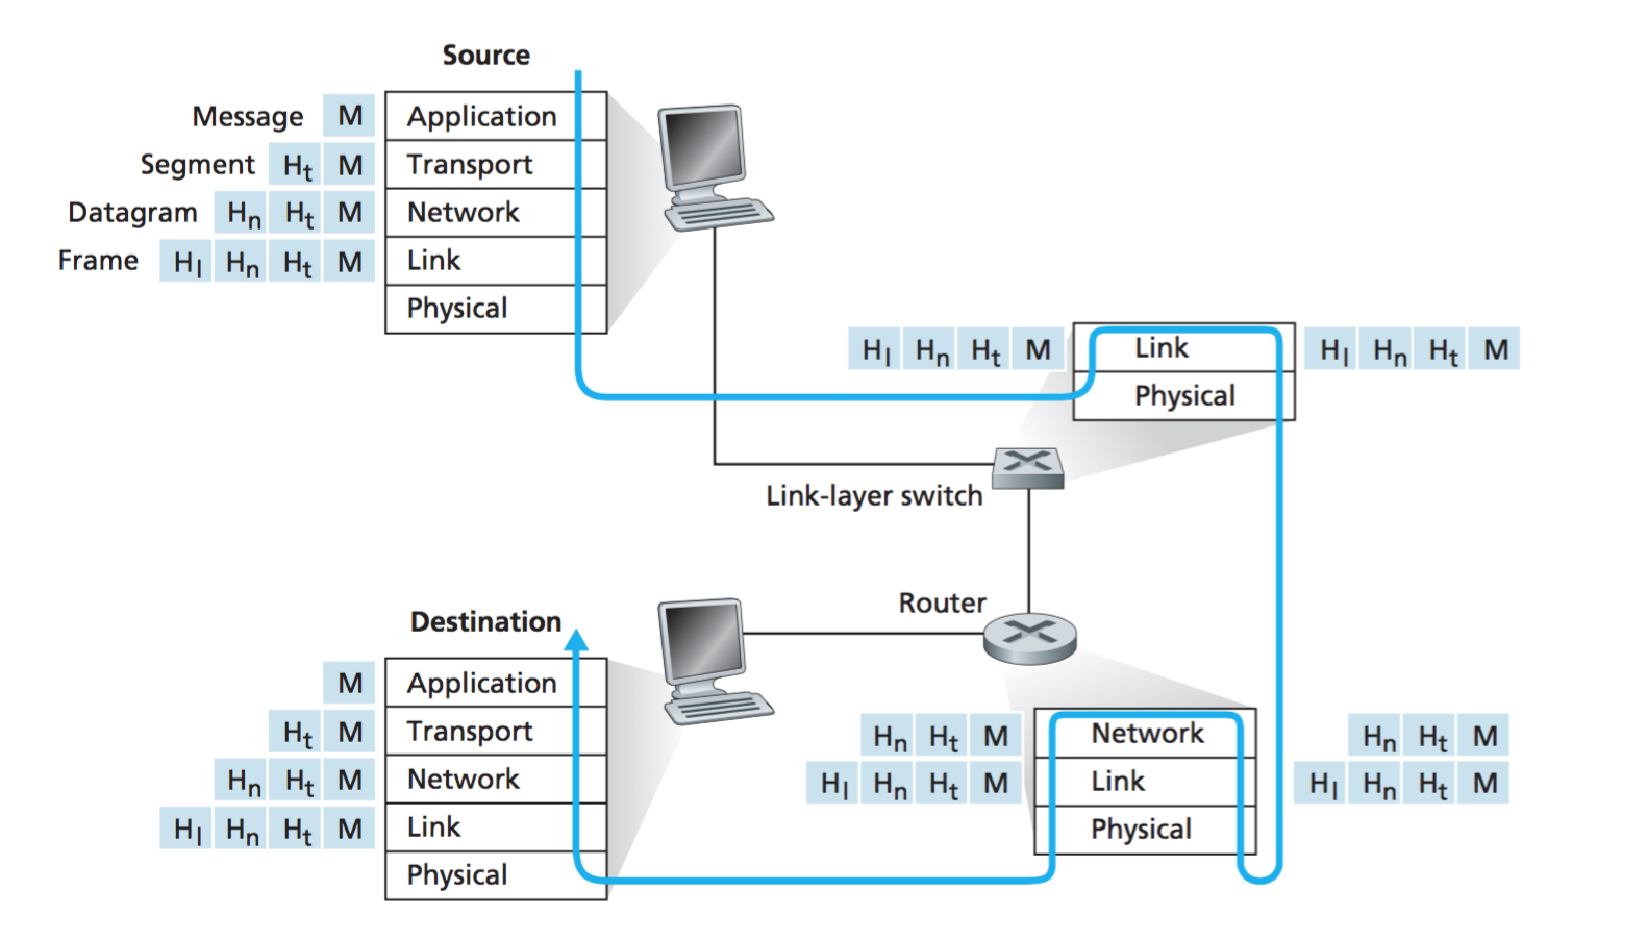
\includegraphics[keepaspectratio=true,scale=0.6]{figuras/encapsulamento.eps}
	\caption[Encapsulamento de mensagens entre camadas \cite{kurose2012}]
          {Encapsulamento de mensagens em um modelo de camadas \cite{kurose2012}}
	\label{fig:encapsulamento}
\end{figure}

A Figura \ref{fig:encapsulamento} mostra este processo no contexto do TCP/IP, também
conhecido como a suíte de protocolos da Internet. Neste caso, os protocolos de cada
camada adicionam um cabeçalho às mensagens recebidas do nível anterior, o que
permite a adição de informações adicionais destinadas ao mesmo protocolo
implementado no comunicante.

O OStatus é outro exemplo de uma suíte de protocolos, por sua vez proposto para a
federação de aplicações, que envolve alguns padrões intermediários na construção de
implementações independentes e interoperáveis. Apesar de não adotar explicitamente
um modelo de camadas, também exemplifica a importância dos conceitos de hierarquia e
encapsulamento na garantia de interoperabilidade.



\section{PADRONIZAÇÃO DE PROTOCOLOS}

A definição de protocolos é apenas o primeiro passo para a intercomunicação de
sistemas. Se não existir um acordo a respeito da especificação utilizada será mais
difícil estabelecer a comunicação entre serviços \cite{kurose2012}. A padronização
garante o estabelecimento deste acordo.

\begin{sloppypar}
O conceito de efeito de rede indica que a adoção de um protocolo se torna mais
valiosa à medida que um maior número de entidades também o utilize
\cite{liebowitz1998}. Justifica-se portanto o interesse em incentivar a padronização
de protocolos.
\end{sloppypar}

A partir do momento em que uma série de entidades entra em consenso a respeito da
especificação de um protocolo, estabelece-se um padrão \textit{de facto}. A
iniciativa de padronização também pode surgir através de entidades regulamentadoras,
como a Organização Internacional para a Padronização (ISO), ou a \textit{Internet
Engineering Task Force} (IETF), o que leva ao estabelecimento padrões \textit{de
jure} \cite{tanenbaum2010}.

O processo de definição de novos padrões \textit{de jure} depende da entidade
regulamentadora relacionada, e ocasionalmente parte de padrões \textit{de facto} já
utilizados na comunidade. Geralmente uma especificação é proposta, discutida, e
revisada pela entidade antes de se tornar um padrão, o que no caso da ISO pode levar
de seis meses a alguns anos \cite{tanenbaum2010}.

Propostas e padrões estabelecidos devem ser documentados de alguma forma. A IETF
adota o formato de \textit{Request for Comments} (RFC), publicações que descrevem
completamente uma especificação, e estão disponíveis a consulta pela comunidade.

Uma proposta deve cumprir uma série de requisitos antes de ser endossado por uma
organização. No caso da IETF, cada proposta passa por vários níveis de maturidade
até alcançar a categoria de padrão. Cada um destes níveis pode ser alcançado ao
satisfazer as recomendações de determinados grupo da comunidade. Um exemplo destes
requisitos é a exigência de uma prova de conceito de interoperabilidade, como uma
implementação de referência entre duas ou mais entidades distintas \cite{rfc1280}.

Protocolos de federação também estão sujeitos ao efeito de rede, e apresentam as
mesmas necessidades de padronização. O \textit{Simple Mail Transfer Protocol} é um
exemplo de especificação utilizado na interoperabilidade de sistemas federados que
passou por um esforço oficial de padronização, tornando-se um caso interessante na
análise deste processo.


\subsection{Simple Mail Transfer Protocol}

\begin{sloppypar}
Um sistema de \textit{e-mails} pode ser considerado federado, já que respeita a
definição de implementações interoperáveis no modelo cliente servidor apresentada
por \cite{barocas2012}. O SMTP é um dos protocolos utilizados na implementação de
interoperabilidade entre serviços distintos.
\end{sloppypar}

Trata-se de um protocolo para o transporte e entrega de mensagens de e-mail entre
processos. A especificação garante que a troca de mensagens aconteça entre clientes
que se localizam em redes diferentes, o que permite a construção de um serviço que
funcione de maneira confiável sobre a internet \cite{rfc2821}.

Caracterizado como um protocolo orientado a conexões entre clientes e servidores, ou
transmissores e receptores, o SMTP é guiado por uma série de comandos predefinidos.
Os servidores também são responsáveis por retransmitir mensagens, caso não sejam os
destinatários finais \cite{kurose2012}.

A troca de mensagens geralmente acontece em um único salto após o estabelecimento de
uma conexão orientada entre o remetente e o destinatário. A retransmissão de
mensagens é uma alternativa, utilizada por exemplo em casos em que um usuário moveu
sua caixa de e-mails de um servidor para outro e deseja receber as mensagens no seu
novo endereço.

\begin{figure}[h]
	\centering
		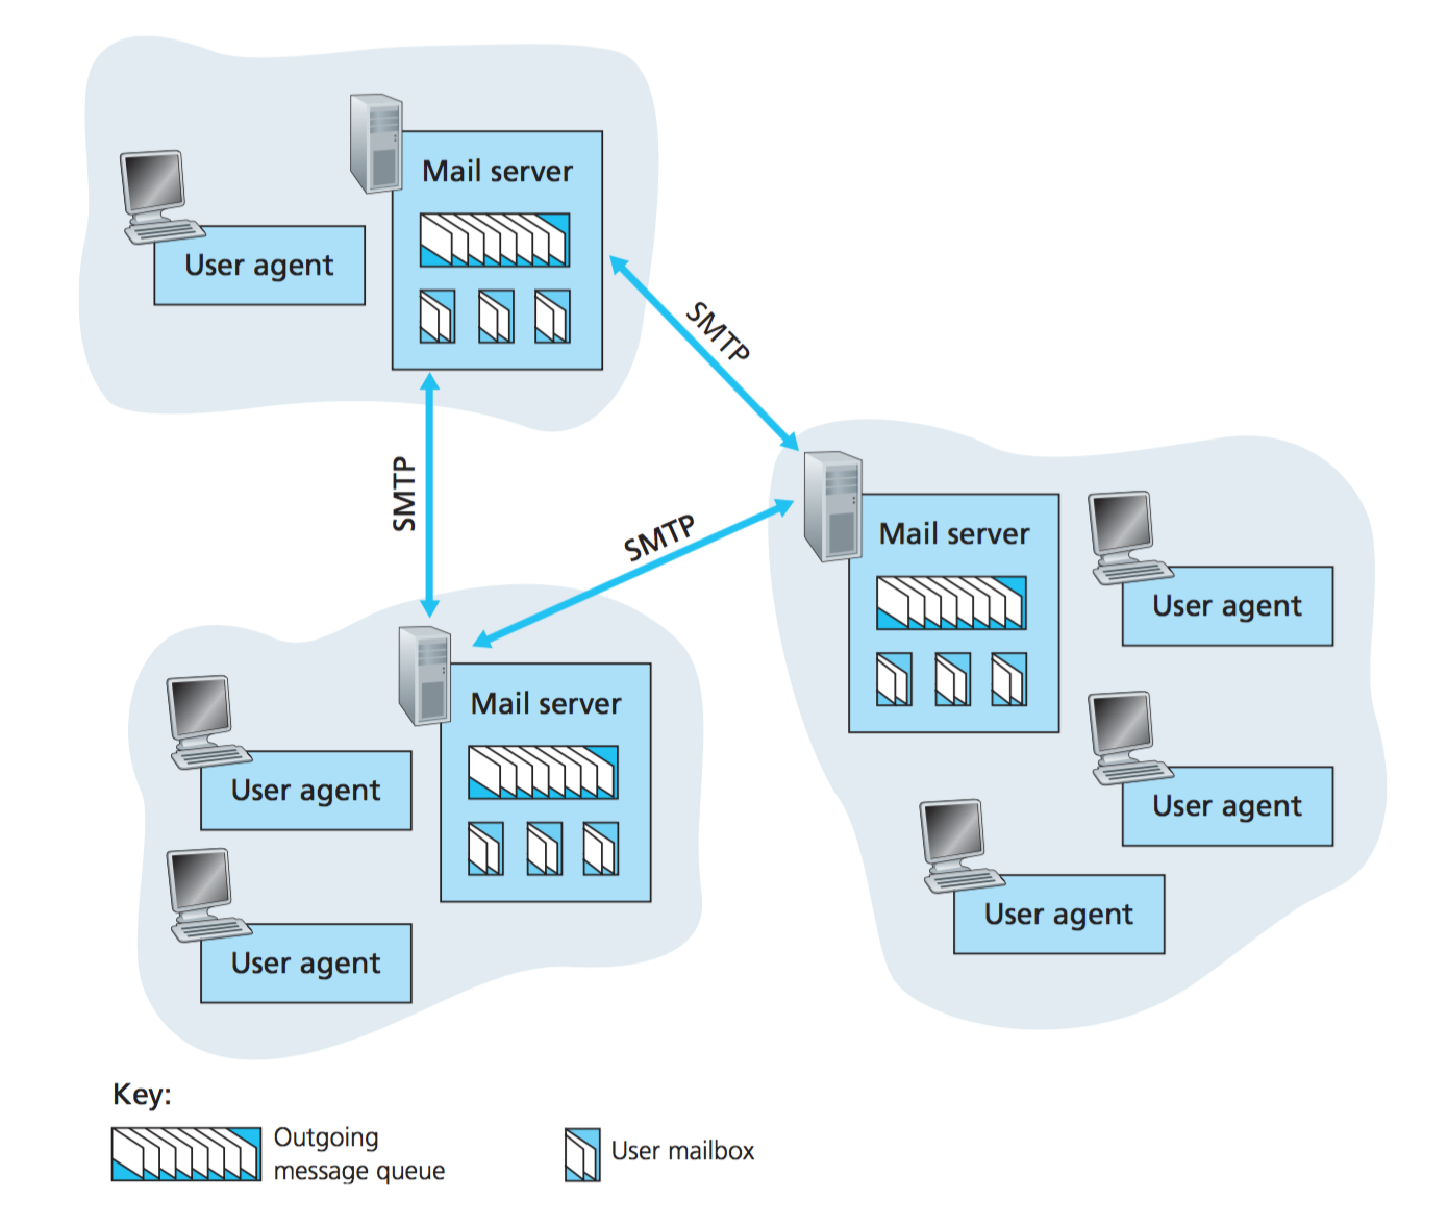
\includegraphics[keepaspectratio=true,scale=0.6]{figuras/smtp_internet.eps}
	\caption{Uma visão geral de um sistema de e-mails \cite{kurose2012}}
	\label{fig:smtpInternet}
\end{figure}

Como pode ser visto na Figura \ref{fig:smtpInternet}, o SMTP é um protocolo
intermediário entre servidores de e-mail que alternam entre os papéis de transmissor
e receptor. Cada um destes servidores fornece a seus próprios clientes, constituindo
sistemas menores onde a interação não é necessariamente coberta pela especificação
do SMTP.

Cada um destes sistemas intermediários não é necessariamente compatível, visto que a
comunicação entre o servidor e o usuário depende das aplicações envolvidas, e
eventualmente utiliza outros padrões, como por exemplo POP3 ou IMAP no gerenciamento
de caixas de e-mail pessoais \cite{tanenbaum2010}.

Por se tratar de uma especificação amplamente utilizada na Internet, o SMTP se
tornou foco de grupos de trabalho da IETF, passando pelo processo de padronização
formal desta entidade, incluindo a publicação em formato de RFC. Trata-se de um
padrão \textit{de jure} aberto, definido por uma organização antes de ser adotado
pelo mercado.

Considerando a descentralização da arquitetura e a padronização do protocolo,
qualquer novo sistema é capaz de implementar e se tornar parte da federação com
relativa facilidade. Nestes casos a heterogeneidade entre os sistemas intermediários
é completamente transparente para os usuários do serviço, o que o indica como um
protocolo de federação bem sucedido.



\section{PROTOCOLOS DE FEDERAÇÃO}

A inexistência de um protocolo padrão para a federação de mídias sociais dificulta
o desenvolvimento de aplicações interoperáveis. São enfrentados os mesmos problemas
identificados na intercomunicação de redes heterogêneas, já que os desenvolvedores
solucionam os problemas com tecnologias diferentes, de acordo com as próprias
restrições e necessidades.

Ainda que exista uma tendência da comunidade em adotar propostas de protocolos, o
que pôde ser observado no caso do projetos OStatus e Diaspora, abordagens
alternativas naturalmente serão desenvolvidas. A ausência de um protocolo bem
difundido segmenta a adoção por parte dos desenvolvedores, o que prejudica o efeito
de rede e impede o surgimento de um padrão \textit{de facto}.

Fazendo um paralelo com o SMTP, o mais próximo a uma entidade como IETF no caso dos
protocolos de federação para redes sociais é o \textit{World Web Consortium} (W3C),
que também endorsa padrões oficialmente por meio de relatórios técnicos. O processo
de padronização tem início com a criação de um grupo de trabalho que deve produzir
rascunhos da especificação, sujeitos à revisão da comunidade pública e dos membros
do W3C. Se um rascunho é revisado o suficiente e cumpre os critérios da comunidade,
pode eventualmente se tornar uma recomendação do consórcio \cite{nevile2015}.

Ao discutir a padronização da federação é interessante não só analisar o esforço da
comunidade em discutir e adotar propostas ainda não completamente estabelecidas,
como também identificar as questões que impediram o acordo. Não existem referências
na literatura que tratam das dificuldades no estabelecimento de padrões para a
federação, e a discussão da comunidade está espalhada por listas de discussão e
repositórios de projetos individuais. Antes de abordar este debate, é importante
apresentar os projetos de federação que ganharam maior visibilidade, o OStatus e o
Diaspora.


\subsection{OStatus}

O OStatus\footnote{\url{https://www.w3.org/community/ostatus}} é um conjunto de
protocolos que permite interação em tempo real entre redes redes sociais. Foi
inicialmente proposto por Evan Prodromou para a implementação do StatusNet, que
posteriormente deu origem ao projeto GNU
Social\footnote{\url{https://gnu.io/social}}.

Até certo ponto, tecnologias como o Atom e RSS permitem a interação entre sistemas,
mais especificamente no compartilhamento de conteúdo. No entanto, são restritas no
que diz respeito a interação em tempo real, problema que o OStatus propõe resolver
combinando \textit{feeds} Atom com uma série de outros mecanismos.

A especificação do OStatus propõe a utilização das tecnologias listadas a seguir.

\begin{itemize}
  \item{PubSubHubbub: mecanismo de inscrição e submissão}
  \item{WebFinger: descoberta de identidade}
  \item{Activity Streams: representação de atividades de usuários em redes sociais}
  \item{Salmon: descentralização de trocas de mensagens}
\end{itemize}

O projeto obteve visibilidade na comunidade, contando com uma das maiores
iniciativas de padronização. O OStatus chegou a se tornar alvo de um grupo de
trabalho do W3C em 2012, uma das maiores organizações de padronização para a
\textit{web}. Apesar disto, o grupo não apresentou avanços desde então, e o
desenvolvimento do projeto está estagnado.

\subsubsection{PubSubHubbub}

O PubHubSub\footnote{\url{https://github.com/pubsubhubbub/PubSubHubbub}} especifica
um sistema distribuído para publicação e assinatura de conteúdos. A ideia é que
serviços possam se inscrever em diretórios centrais (ou \textit{hubs}), expressando
o interesse em receber as atualizações em tempo real. Este padrão complementa
tecnologias como o RSS, que baseia a atualização apenas na solicitação dos
interessados.

Serviços inscritos devem identificar o tópico desejado através de URIs, e oferecer
um servidor disponível pela internet para que a notificação seja realizada. É de
responsabilidade de cada serviço notificar os \textit{hub} conhecidos a cada nova
publicação. Cada \textit{hub} é responsável por replicar a mensagem a todos os
serviços inscritos.

\subsubsection{WebFinger}

\begin{sloppypar}
O WebFinger é um protocolo de descoberta de identidade que soluciona o problema do
compartilhamento de informações de usuários entre servidores remotos \cite{rfc7033}.
A proposta é que a partir de um atributo identificador e do endereço do servidor de
origem, seja possível garantir existência de um usuário e recuperar suas informações
públicas.
\end{sloppypar}

A especificação do WebFinger propõe que todos os recursos possam ser identificados
por uma URL, e que todas as solicitações e respostas sejam realizadas através de
requisições HTTP. Servidores que forneçam informações através do WebFinger devem
responder aos \textit{endpoints} definidos no protocolo com objetos JSON. Servidores
que pretendam consumir tais informações precisam conhecer apenas a URL do recurso de
interesse, o que pode ser encontrado a partir do identificador do usuário e do
domínio do servidor de origem (em um processo que pode ser classificado como LRDD
\cite{lrdd2010}). 

\subsubsection{Activity Streams}

O Activity Streams\footnote{\url{http://activitystrea.ms/}} é uma especificação que
propõe um formato para a representação das atividades dos usuários em uma rede
social. O objetivo é facilitar o consumo destas ações para o resto da rede e
serviços externos.

A especificação mais atual do Activity Streams propõe a representação em formato
JSON, definindo propriedades que identificam a ação, o usuário responsável, e a
entidade alvo. Especificações mais antigas utilizam o padrão Atom, com restrições
semelhantes em relação ao conteúdo das mensagens. O OStatus adota a especificação
baseada em Atom, utilizando mensagens em formato XML.

O padrão trata apenas da representação das mensagens, dependendo de outros
mecanismos para a distribuição das atividades. Geralmente são utilizadas APIs ou
\textit{feeds} em conjunto com mecanismos de inscrição.

\subsubsection{Salmon}

Combinar soluções como Atom e PubHubSub permite que conteúdos sejam publicados e
atualizados em tempo real. No entanto, a partir do ponto em que um conteúdo pode ser
consumido e atualizado a partir de um número arbitrário de serviços, também deve-se
investir esforço para garantir que o seu estado seja o mesmo em toda a rede.

O objetivo do Salmon\footnote{\url{http://www.salmon-protocol.org}} é descentralizar
a capacidade de contribuir com o estado de um conteúdo, mas mantendo sua
consistência por toda a federação. Para isto, especifica a troca de mensagens entre
o servidor de origem e todos os outros que podem contribuir com o estado de um
conteúdo, definindo o formato das mensagens, e as diretrizes necessárias para
agregar as atividades.

Um servidor que implemente o protocolo deve incluir a URL de um \textit{endpoint}
capaz de processar mensagens Salmon, enviadas para este endereço por qualquer
serviço interessado em modificar o estado de uma publicação. Uma mensagem Salmon se
trata de uma nova entrada no \textit{feed}, codificada em \textit{base64} e envolta
por outra estrutura envelope (geralmente XML) assinada digitalmente. Cabe ao
servidor processar as solicitações de acordo com suas próprias políticas.

\subsubsection{Estado do padrão}

O projeto OStatus deu um passo importante em direção à padronização com a criação do
grupo de trabalho no W3C. No entanto, a comunidade não conseguiu entrar em consenso
em relação às decisões do protocolo, principalmente no que diz respeito à
privacidade.

Não exitem avanços no projeto nos últimos anos, e o grupo de trabalho do W3C não
produziu nenhum relatório desde que foi criado. Em 2012 o fundador do projeto, Evan
Prodromou, anunciou o desenvolvimento do \textit{pump.io}, outro protocolo de
federação, abandonando o desenvolvimento do OStatus.

Ao mesmo tempo em que não existia comunidade ativa para a evolução do projeto, parte
das tecnologias utilizadas continuou a ser mantida, o que contribui para o seu
estado de obsolescência. O Activity Streams, por exemplo, já conta com uma segunda
especificação que suporte tecnologia JSON, enquanto o OStatus ainda considera a
especificação baseada em Atom.

Apesar de defasado, o OStatus ainda é usando em novas iniciativas de redes sociais
livres e federadas. O Mastodon\footnote{\url{https://github.com/Gargron/mastodon}} é
um exemplo de projeto moderno, atualmente em desenvolvimento, e que optou pela
compatibilidade com o GNU Social através da suíte do OStatus.


\subsection{Diaspora}

O projeto Diaspora\footnote{\url{https://diasporafoundation.org/}} surgiu com a
intenção de implementar o conceito de redes sociais descentralizadas em resposta aos
problemas de liberdade e privacidade encontrados em plataformas sociais privadas.
Sua primeira versão foi lançada em Setembro de 2010 como fruto de uma campanha de
financiamento coletivo, passando a ser completamente governado pela comunidade a
partir de Agosto de 2012.

A proposta dos desenvolvedores é evitar a centralização de conteúdo, portanto a
falta de controle sobre as informações, construindo uma rede de instâncias pessoais
da plataforma, ou \textit{pods}. Cada servidor Diaspora reúne apenas as informações
dos seus próprios usuários, mas em cooperação com outros \textit{pods} possibilita a
interação em uma rede federada.

O protocolo de federação do Diaspora foi definido para convergir com o OStatus assim
que o último passe a suportar o conceito de privacidade limitada, o que nunca
aconteceu. A implementação leva em consideração a troca de mensagens em formato XML,
respeitando alguns conceitos básicos como a existência de usuários remotos e
atualização remota e retransmissão.

\subsubsection{Usuários Remotos}

Um conceito fundamental para a implementação de redes federadas é considerar a
existência de usuários remotos. A maioria das aplicações só possui o conceito de
usuários locais, que estão diretamente autenticados no serviço e possuem todas as
informações na base de dados local. No entanto, ao possibilitar a interação com
usuários de outras redes, usuários externos ao sistema precisam ser explicitamente
considerados na implementação das funcionalidades.

O Diaspora conceitualiza seus usuários em locais e externos. Enquanto usuários
locais respeitam a definição tradicional, os usuários externos interagem com a
aplicação através dos mecanismos de federação. É importante prever a existência de
usuários externos na modelagem de sistemas. Por este motivo, implementar federação
em aplicações já consolidadas pode exigir um certo esforço de refatoração.

\subsubsection{Capacidade de Retransmissão}

A retransmissão é essencial em sistemas federados, visto que interações em uma rede
eventualmente devem afetar \textit{pods} relacionados. A restrição implementada pelo
Diaspora indica que todas as notificações neste contexto sejam entregues tanto aos
usuários locais quanto aos usuários remotos. Adicionalmente, a notificação de
usuários locais não deve depender da resposta dos demais \textit{pods}.

Em configurações de integração mais complexas, a capacidade de retransmissão passa a
ser um requisito essencial para a troca de mensagens. Considere uma situação
hipotética em que \textit{pods} \textbf{A} e \textbf{B} são federados com o
\textit{pod} \textbf{C}, mas não entre si. Qualquer modificação em um conteúdo de
\textbf{C} compartilhado com \textbf{A} e \textbf{B} deve afetar os três
\textit{pods}. No entanto, se a modificação partir de \textbf{A}, há uma dificuldade
em notificar \textbf{B}, visto que o \textit{pod} em questão só reconhece a
existência de \textbf{C}. A solução defendida pela implementação do Diaspora é que
\textbf{C} retransmita a notificação para todos os \textit{pods} com os quais o
conteúdo seja compartilhado. Isso garante que todos os sistemas federados envolvidos
em uma interação sejam notificados, contribuindo com consistência das informações.

\subsubsection{Troca de Mensagens}

O Diaspora define um conjunto de mensagens que delimitam as possíveis interações
entre \textit{pods}.

\begin{itemize}
  \item{Compartilhamento de informações}
  \item{Publicações de conteúdo}
  \item{Comentários e reações a publicações}
  \item{Mensagens privadas}
\end{itemize}

A troca de mensagens segue a definição do protocolo Diaspora, que utiliza um
subconjunto do protocolo Salmon. De modo geral, restringe como a mensagem deve ser
construída e enviada para o \textit{endpoint} Salmon do \textit{pod} de destino. 

\subsubsection{Estado do protocolo Diaspora}

A partir de 2012 o projeto passou a ser completamente mantido pela comunidade, logo
após que os fundadores abandonaram o projeto. Apesar disto, ainda conta com
desenvolvimento ativo. O protocolo também continua a ser mantido, sendo que a
especificação mais recente foi lançada em Julho de 2016.

O projeto ganhou certa visibilidade pouco após a sua proposta, mas o protocolo não
foi capaz de adquirir adoção o suficiente para desencadear uma tentativa formal de
padronização. Ainda assim, é oficialmente suportado por outras redes sociais como o
Friendica, o Hubzilla e o Loomio.

O protocolo ainda não foi capaz de padronizar a comunicação entre quaisquer redes
sociais genéricas, tendo servido apenas ao propósito de permitir a integração
de qualquer outra rede com o Diaspora.


\subsection{Padronização de protocolos de federação}

Apesar de não existirem produções acadêmicas que explorem a inexistência de um
protocolo padrão para a federação de redes sociais, todo o debate da comunidade está
documentado em lista de discussões e grupos de desenvolvimento. Esta seção é fruto
de uma análise subjetiva baseada no conteúdo destes repositórios, e pretende
discutir os fatores que levaram à segmentação dos projetos de federação e no
insucesso de alcançar um padrão.

A comunidade destaca duas estratégias diferentes para alcançar
federação\footnote{Parte da discussão está registrada em listas de \textit{e-mail},
como por exemplo em uma das \textit{threads} da lista de redes sociais federadas do
W3C, que pode ser visualizada em
\url{https://lists.w3.org/Archives/Public/public-fedsocweb/2013May/0058.html}}.
Primeiro, a manutenção de um protocolo ou sistema que deva ser suportado por todas
as aplicações interessadas em ingressar na federação, um método caracterizado por
uma entidade que é o denominador comum entre todas as redes.

A segunda estratégia é que aplicações implementem explicitamente o protocolo de cada
rede com a qual se deseja integrar, o que descarta a necessidade imediata de um
protocolo padrão, configurando uma técnica poliglota.

A estratégia poliglota apresenta restrições à federação de sistemas, já que depende
que cada aplicação responda aos protocolos de todas as outras aplicações da rede.
Esta estratégia parece incentivar a segmentação de especificações, ao contrário do
que aconteceria com a utilização de um único protocolo como denominador comum. Por
outro lado, a utilização de um denominador comum depende de um único protocolo capaz
de cobrir as restrições de todas as possíveis redes, visto que cada aplicação propõe
seus próprios conceitos a respeito de relacionamento de usuários, publicação e
compartilhamento de conteúdos, e privacidade.

As críticas direcionadas ao OStatus em relação a privacidade dos
conteúdos\footnote{As críticas também pode ser vista na lista de \textit{e-mails} do
W3C \url{https://lists.w3.org/Archives/Public/public-fedsocweb/2013May/0061.html}} é
um exemplo das barreiras que podem ser causadas por estas diferenças conceituais.
Visto que o projeto suporta apenas conteúdos públicos, redes que possuam uma
definição de privacidade mais complexa não são atendidas. Ao mesmo tempo em que o
OStatus falhou em satisfazer estas necessidades, projetos que deram maior atenção à
privacidade emergiram e ganharam visibilidade, como o Diaspora e o Friendica.

Uma especificação que atenda universalmente todas as redes sociais exigira um grande
esforço de projeto, desenvolvimento e manutenção. Uma alternativa seria um protocolo
que definisse apenas um subconjunto de políticas que serviria como base para todas
as implementações. Todavia, estes conceitos precisariam ser elementares o suficiente
para cobrir políticas específicas que eventualmente são opostas, fazendo com que as
comunidades não fossem capazes de chegar a um acordo por causa de seus próprios
objetivos ou filosofias.

Apesar do limite que ser introduzido por um protocolo que especifique apenas um
conjunto de diretrizes para interações entre usuários, cada aplicação poderia
resolver suas necessidades específicas com base nas restrições do denominador comum,
formando uma suíte de protocolos organizada em um modelo de camadas. A distribuição
de responsabilidade nesta hierarquia de protocolos possibilitaria a utilização de um
denominador comum diminuindo o impacto das restrições sobre os objetivos e decisões
arquiteturais de aplicações que o adotassem. No entanto, a adoção não só dependeria
de um acordo por parte das comunidades como envolveria a reformulação de todos as
redes sociais existentes, o que não contribui para a viabilidade desta estratégia.

A adoção de uma estratégia de certa forma contradiz a necessidade de padronização
observada em redes de comunicação. Neste caso, parece claro que a dificuldade em
encontrar um acordo na integração das redes sociais ultrapassa os benefícios da
interoperabilidade que seriam resultado da adoção de um padrão. Por outro lado, se
mais aplicações implementam a integração individualmente projetos específicos podem
se destacar, o que desencadearia um efeito de rede, e conduziria a um padrão válido
para um subconjunto de aplicações.

Por enquanto o caminho para a federação é adotar a especificação de um dos projetos
existentes, que geralmente é definida a partir de uma suíte de padrões já
estabelecidos. A escolha deve ser feita levando em consideração a atividade da
comunidade e a aderência da especificação às necessidades particulares. A comunidade
do Noosfero identificou que esta especificação é a proposta pelo Diaspora.

Partindo dessa definição, deve-se prosseguir com o projeto da federação no Noosfero
através do protocolo Diaspora, o que cobre a implementação dos conceitos necessários
em sua arquitetura e a utilização de um conjunto de padrões já estabelecidos na
promoção da interoperabilidade.
